% !TeX spellcheck = en_GB
\chapter{Time and Distance}\label{ch:distancetime}

Like for any martial art, time and distance are most essential notions to fencing.
It is only by mastering them that one may hope to become a truly proficient fencer.

Intricately intertwined, these two concepts are not absolute nor fixed notions though and bear all but no relation with actual physical dimensions.
While they do help describing and objectively commenting fencing actions,
they also encompass the sense of time and distance in a context of confrontation, that is to say the perception that the opponents have of their relative capacities of action.
As such, time and distance are central to fencing tactics and strategy.

\section{Fencing time} \index{fencing time}
\emph{Fencing time} is a unit of time defined as the duration of a simple action: a step, a cut, a thrust, a parry, etc.\index{simple actions}
The number of time units taken by a combined action is the number of consecutive simple actions that compose it, simultaneous simple actions counting for one unit of time only.
For example, one step while parrying followed by a riposte would sum up to two time units in all.

Fencing time is not related to actual clock time, it is not a definite span of time since the actual duration of a simple action will depend upon the speed at which it is executed.
Fencing time is rather related to the notion of commitment in an action associated with an underlying intent.\index{intention}\index{transformation}
As long as the fencer is not fully engaged in his action, he may still transform and change his intent during the same unit of time.
It is only after full commitment that it becomes impossible to interrupt the course of the ongoing action and change one's mind during the same fencing time.
This does not mean though that an action must necessarily be led to its term as soon as it has been initiated but that transformations take more time when the intention is fully engaged.

This very important tactical notion is used in feints and false attacks.
As we shall see further, when feinting, full commitment is not sought but the fake strike must be convincing enough to compel the opponent to get fully involved in parrying what he thinks to be an attack.
It is then possible to modify our initial action during the same time and launch the true attack while the opponent, sticking to his first reaction, is baffled.
As a general rule, it should be avoided to engage in action too early so as to preserve for as long as possible a capacity to transform and adapt effectively to the opponent's reactions.

Fencing time may thus be seen as a useful theoretical notion for assessing the fencers' current ability for initiative, transformation or response during actions. 
It helps to formalise the course of simple actions when studying a \emph{phrase d'arme}, no matter how fast or slow it is performed and assuming that both opponents are equally fast.
Of course, in real life, some fencers are faster than others but actually, speed does not matter. Only tempo is important: what really counts is the right action at the right time.
It is always possible to compensate for a lesser speed with the effective use of techniques and tactics, and above all, by mastering rhythm.\index{rhythm}
A faster fencer may loose his advantage if he is forced by a proficient opponent to use more fencing times for his actions.
This is sometimes adopted as a strategy by some fencers who keep their opponent in a constant state of urgency while allowing themselves to take their time.
Whether they do so by maintaining a permanent threat against their opponent or by always stepping out of his lines of attack, they impose their own rhythm on the fight and do not allow their opponent to regain the initiative.
To achieve this goal however, it is essential for them to stay connected to their opponent and that every single move and menace perfectly fits his reactions.
In other words, the rhythm of the fight is actually a combination of the rhythms of both opponents.
Although, the rhythm of one fencer may take precedence over the other's it never does so independently: connection and relationship are essential.

The ability to grasp and match the rhythm of our opponent while concealing our own is therefore fundamental to seize the right moment and gain an advantage.
It is essential to maintain a constant awareness of the opponent's moves and not to get trapped into heedless anticipation by misleading regular rhythm patterns. 
Great care should be paid too not to embrace too regular a rhythm that would consequently be easily predictable by the opponent. 
Controlling rhythm does imply a relaxed state of mind ensuring we are constantly ready to adapt to the situation and transform it to our advantage by responding to the opponent's moves unexpectedly.
More than quick reactions though \textemdash{} haste should not be mistaken for speed \textemdash{} this is definitely a question of being on the edge of a perpetual present, letting the past flow away and the future happen without clinging to any premeditated technique.

\section{Distance and measure} \index{distance}
Just as fencing time does not actually represent an objective span of time, the effect of the distance between the two opponents on their respective ability to strike each other is more important here than their actual distance.
We thus define measure \index{measure} as the distance range within which it is possible to hit the opponent in one fencing time.
In other words, it is a distance close enough for not requiring more than one step to strike.
If at least two steps are necessary, we are said to be out of measure.

On this basis, three in-measure distances may be defined:
\begin{enumerate}
\item \emph{Guard distance} or \emph{long measure}: one step is required for striking. This is the most usual distance in free play as it offers a good compromise between a protective attitude and a more pressing one.
\item \emph{Reach distance} or \emph{short measure}: at this distance, it is possible to strike with the appropriate section of the blade without having to step forward nor backward.
\item \emph{Close distance}: this distance is too short to use the blade effectively, only close combat techniques can be used such as kicking, punching, grappling, etc.
\end{enumerate}

But there is much more to measure than distance.
Measure is influenced indeed by the fencers' stances and their respective angles of attack.
The guard and foot position determine the range that can be covered by the sword during one fencing time with simple actions: step, weight transfer, arm and body rotation. \index{simple actions}
Whether the target being aimed at actually lies or not within this range and may be reached in one time by an effective cut or thrust will in turn mainly depend upon the angle of attack and the opponent's cover.

It should be reminded that both the angle of attack and the sword's range must be considered here not only in the horizontal plane but in three dimensions, the longest distance being attained with the arm fully extended horizontally at shoulder level.
Thus, in any situation, the closest targets are those approximately lying at shoulder's height, that is, most of the time, the upper chest and the throat.
Lower targets may be reached by stepping forward but also by crouching or leaning so as to lower the shoulder down to target level.

Figure \ref{fig:distance_stance} shows how the sword's range is affected by the fencer's stance and stepping as well as by the height of the target.

\begin{figure}[h]
\centering
	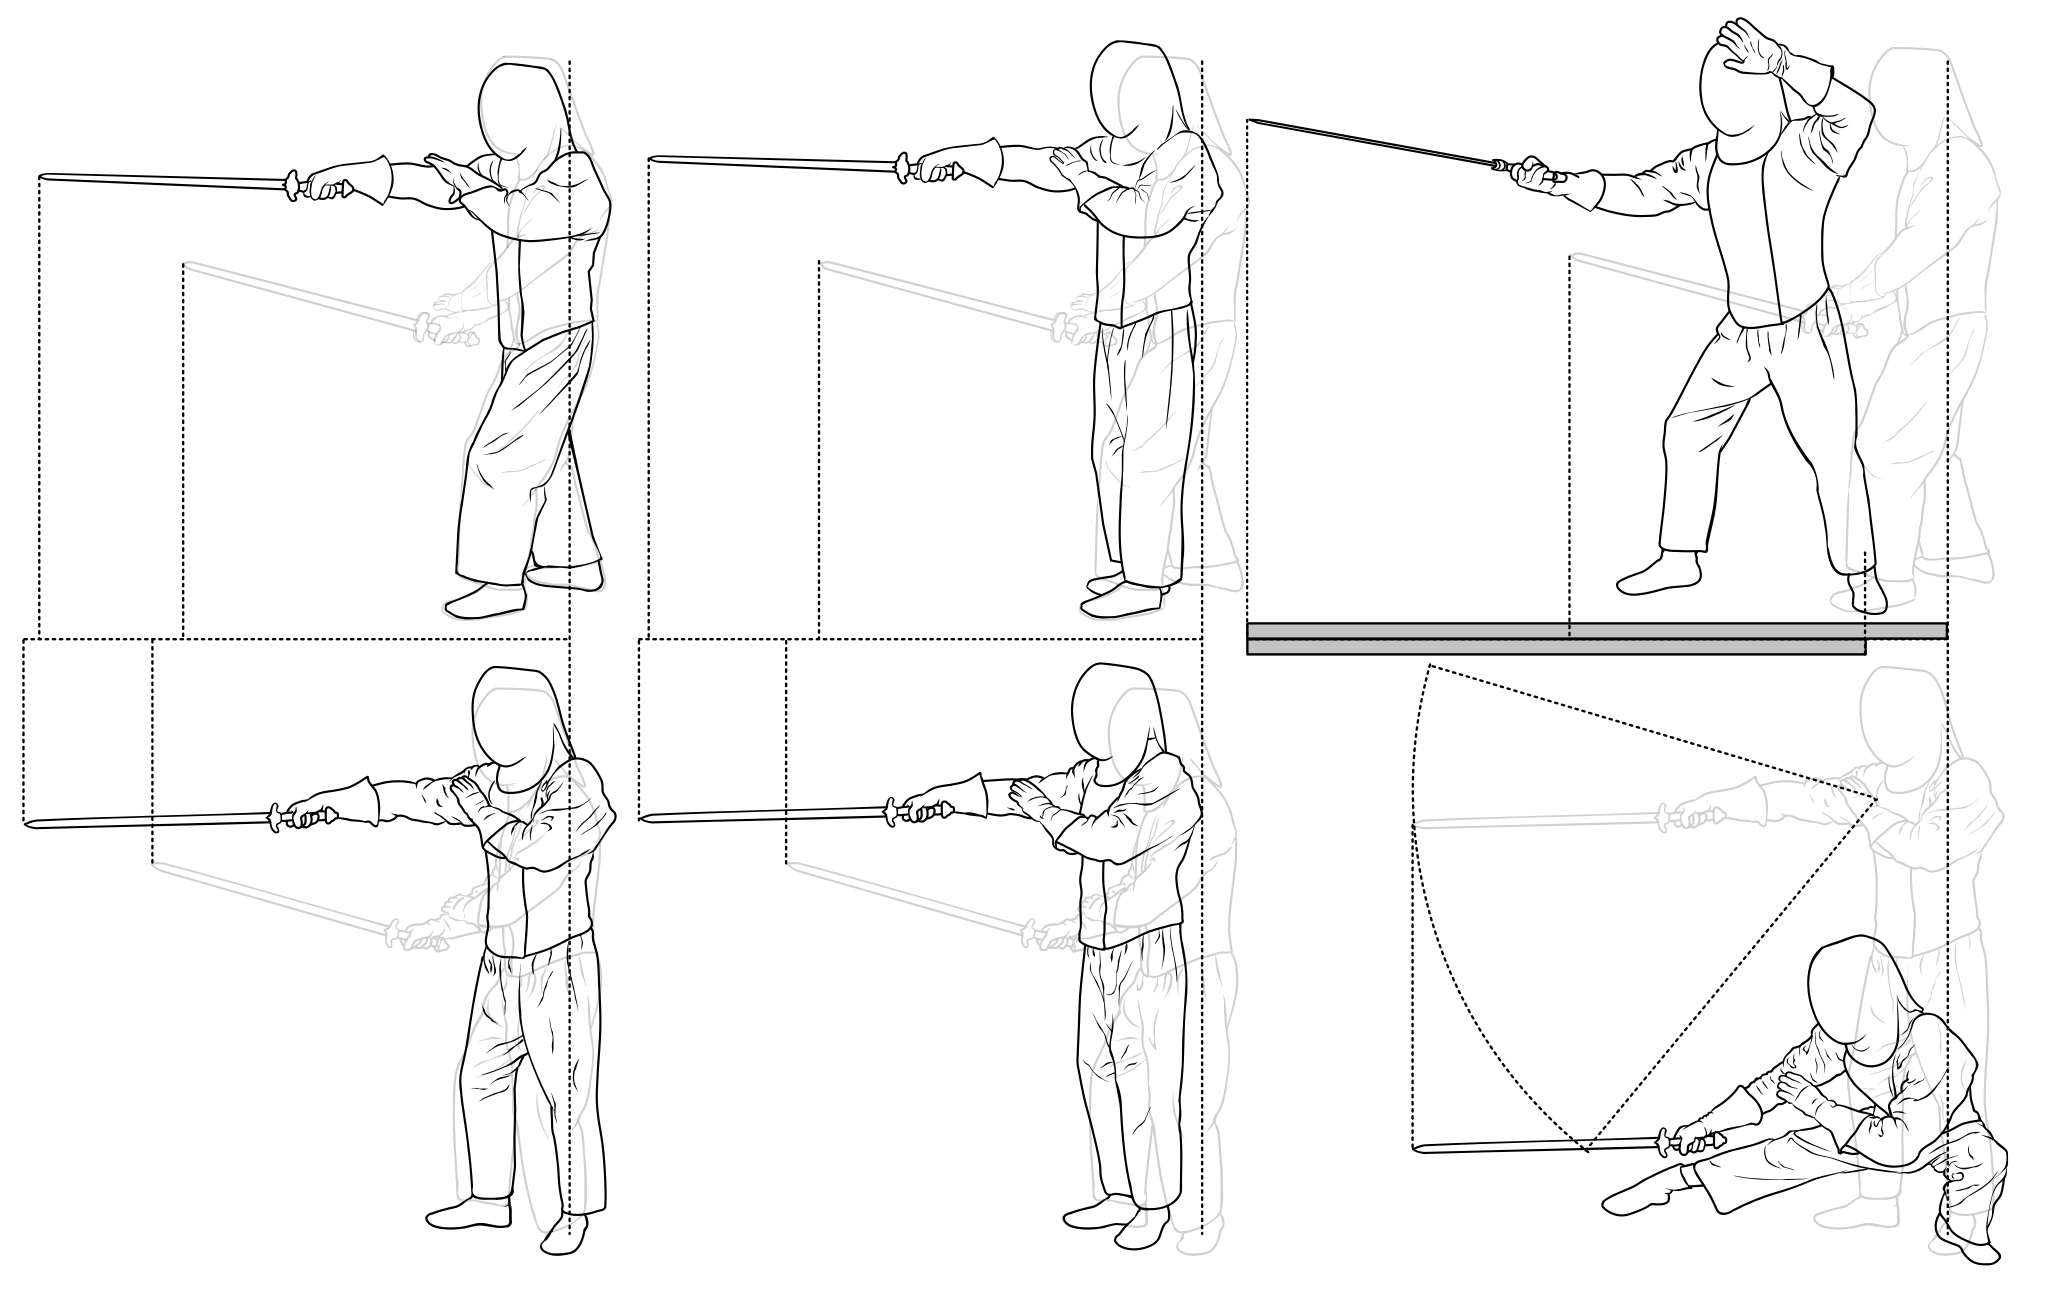
\includegraphics[width=1.0\textwidth]{../../Images/DistanceTime/distance_stance.pdf}
	\caption[Stance and measure]{Some examples of stances and their thrusting range.
	
	The leftmost column shows the distance reached by extending the arm from the initial guard position (drawn in grey). This distance is slightly longer with the right foot forward (bottom figure) because of the larger turning range of the body pushing the sword further. This can also be observed on the guard position which extends slightly further with the right foot in front. The same remark holds for the middle column showing the range attained by extending the arm and closing the step. This difference is smaller though because of the shorter distance between the feet. 
	
	The top right figure shows the maximum range that can be reached with a thrust. Thus, the upper grey box represents the length of the measure when starting with the left foot forward. Thanks to the shifting of the axis to the left foot and the subsequent passing step, this measure is longer than when starting directly with the right foot forward.
	
	In the bottom right figure, the portion of circle represents the vertical range of the sword when standing up without stepping. Even though they may be at the same horizontal distance from the body axis, lower targets may none the less be out of reach unless crouching so as to bring the shoulder at their level.   
	
	All figures are drawn to scale.}
	\label{fig:distance_stance}
\end{figure}

Fencing being dynamic by nature, measure must be further accounted for in an ever changing context and may vary dramatically with every single move of the opponents.
As stepping away from the target increases distance, one may be close enough to be statically in measure, but may be at the same time out of measure if evaluated dynamically.
The combination of time and distance reduces or increases the relative duration of of fencing of fencing time units for each opponent depending on whether their steps bring them closer to or further from their target.

%\begin{figure}[ht]
%\centering
%	\includegraphics[width=0.69\textwidth]{../../Images/EmptyFig.pdf}
%	\caption[Motion and measure]{Motion and measure}
%	\label{fig:distance_motion}
%\end{figure}

The concept of measure is not symmetrical indeed and the opponents are not necessarily within the same measure relatively to each other due to different stances, relative moves or respective angles of attack. 
%As shown in figure \ref{fig:distance_motion}, 
A fencer may thus leverage the asymmetry of measure by stepping towards a direction and from an angle that would dynamically keep his opponent out of measure while simultaneously allowing himself to hit.
\FloatBarrier

This is actually a key to efficient \Taiji{} fencing: the opponent is overcome by the appropriate move at the appropriate time and distance, not by a greater speed.
The principles are respected and the fencer's moves can thus be calm and his mind serene.
It is therefore fundamental to develop an ability to instantly perceive one's own measure as well as the capacity of the opponent to hit so as to constantly adapt to the opponent's moves and strike him on the spot when it is possible to do so while keeping away from his threat.

\section{Drills and exercises}
The following drills and exercises will allow you to apprehend and practice the sense of distance and time.

\subsection{Still target}
This drill is adapted from the one called \emph{tirer au mur} in western fencing.
It consists in aiming thrusts or cuts at a non-moving target.

Take place in front of the target at a long-measure distance, draw a thrust or a cut at the target with one step. 

Repeat this drill starting from various foot positions until you have a good grasp of the long measure in all stances.

Then, you may try yourself at the dynamic version of this drill.
Instead of starting directly in measure, start now from a longer distance requiring more than one step to bring you in short measure.
Approach and strike at the target without interruption, while stepping.

Practise this drill slowly at first and increase your speed gradually, but do not go faster as long as you need to reduce your speed or mark a stop before aiming at the target.
The goal here is to acquire the capacity to evaluate the distance while approaching the target and hit as soon as you are at the appropriate distance.

To increase difficulty, you may also vary the angles of attack and approach in sinuous lines.

Ideally, in order to avoid hard shocks and account for penetration of the blade, the target should yield to hits.
Clothes-pegs on a clothes-line hung at throat level make pretty suitable targets in this regard.

\subsection{Moving target}
This drill is adapted from Olivier Delannoy.
It should be practised with secured blades exclusively and the partner holding the target should at least wear a fencing mask.
You will also need a portable target such as a wooden plank with handles, a table tennis racket or a boxing pad.

The partner holding the target moves around facing the partner carrying the sword, keeping the target turned toward the floor.
The latter follows the stepping of the former, trying to stay in measure.
The target holder may raise the target at any time.
At this signal, his partner must draw a thrust at the target if he is at the appropriate distance.

With a boxing pad or a racket, it is also possible to practice this drill with cuts.

\subsection{Double threat}
%It was inspired by a drill proposed by Keith Farell.
This exercise should be practised very slowly with secured blades and fencing masks.
Full protective gear would be required should the partners decide to play faster.

One partner assumes any stance or guard that may please him and his two partners take a threatening position in measure.

The first partner must then find a way to evade the threats and stay out of the measure of both his partners while hitting at least one of them.

Both threatening partners should stay still for the whole duration of the exercise.
However, in a variant of this drill, they may move slowly, at the same pace as the first partner, to check he really is at a safe distance.

The partners should always take their time in this exercise so as to be able to analyse the situation and practice safely. 

This exercise may be practised with more than three partners.

\subsection{Multiple attackers}
This exercise should be performed imperatively with secured blades and full protective gear.

One partner must defend against the continuous attacks from several partners.
His goal is to deal with as many successive attacks as he can.

Each attack must be launched as soon as the defender has parried the previous one and riposted, but not before.

Attackers should fully engage in their attacks and not try to adapt to the defender's parries.

When responding to an attack, the defender must keep control of his distance to other attackers in order to maintain them out of measure and thus ensure he has enough time to react to their attacks.

\newsavebox{\todoDistance}
\sbox{\todoDistance}{
Include the following in the first figure caption.

This kind of stepping is encountered several times in the Kunlun sword routine, accompanied by an extension of the arm, under the form of a chasing step or a half step preparing a subsequent passing step of the left foot.
On the other hand, when on the left

When in regular stance, right foot forward with the weight on the left foot, advancing brings the weight above the right foot, thus gaining the few inches that were mising to reach the target.
When in crossed stance for instance, a forward passing step of the right foot will bring the whole right side of the body forward, and the sword along with it.
It will thus be possible to hit in one time from much further than if starting with the right foot in front since a passing step of the left foot will not as much allow the sword to simultaneously near the target (see figure \ref{fig:distance_passing_step}).
At close distance, a backward passing step into the crossed stance would bring the sword tip back in front of the opponent's body and ready to thrust.
Figure with different stances and hitting range: better than obcure explanations in the text.


...
? paragraph on strategy and tactics and time and distance
no, the reverse: a paragraph on time and distance in the chapter about strategy

A tall fencer will be in measure at a larger distance, just as someone who has a longer blade. 
Their close distance will also be larger though, which may not be an advantage.

For instance, by assuming an opposite guard, it is possible be at reach distance inside the guard of the opponent who consequently is at close distance: we can thrust at our opponent whereas he cannot use his weapon effectively.
An evident strategy based on these premises consists in progressing gradually towards the reach distance while maintaining the opponent out of measure or at worse in his guard distance.

When in guard distance, mobility should be favoured in order to explore the situation and search for openings in the opponent's guard where it would be possible to enter and hit in one time. The uncovered side is mobile and can dodge if the opponent works his way around our guard and attacks. Mobility is most important so as not to offer a still and easy to reach target.
Ideally, at guard distance, a complete back stance should place us out of measure. Thus, this distance provides a good compromise between safety and the capacity to hit.
In reach distance, we should try and find an opportunity to hit by approaching as much as necessary while keeping the body as far as possible and above all, covered and well protected.
}
